\documentclass[preview]{standalone}

\usepackage{amsmath}
\usepackage{amssymb}
\usepackage{tikz}
\usepackage{float}
\usepackage{xcolor}
\usepackage{stellar}
\usepackage{definitions}

\begin{document}

\id{differentiation-interpretation}
\genpage

\section{Interpretation}

\subsection{Rate of Growth}

\begin{snippet}{calculus-rate-of-growth-interpretation}
Since the derivative \(f'(x)\) represents the rate of change of \(f(x)\),
assuming that \(f(a)\) is defined.
\begin{itemize}
    \item If \(f'(a) > 0\), then \(f(x)\) is increasing at \(x=a\)
    \item If \(f'(a) < 0\), then \(f(x)\) is decreasing at \(x=a\)
    \item If \(f'(a) = 0\), then \(f(x)\) is critical at \(x=a\)
    \item If \(f'(a)\) is not defined, then \(f(x)\) is critical at \(x=a\) (sharp corner)
\end{itemize}
A critical point is when the \function is stationary.
\end{snippet}

\begin{snippetdefinition}{increasing-function-definition}{Increasing Function}
    A \function \(f(x)\) \textit{increases} on an interval \(I\) if
    \[
        \forall x_1, x_2 \in I, x_1 > x_2 \implies f(x_1) \geq f(x_2)
    \]
\end{snippetdefinition}

\begin{snippetdefinition}{decreasing-function-definition}{Decreasing Function}
    A \function \(f(x)\) \textit{decreases} on an interval \(I\) if
    \[
        \forall x_1, x_2 \in I, x_1 > x_2 \implies f(x_1) \leq f(x_2)
    \]
\end{snippetdefinition}

\begin{snippetdefinition}{strictly-increasing-function-definition}{Strictly Increasing Function}
    A \function \(f(x)\) \textit{strictly increases} on an interval \(I\) if
    \[
        \forall x_1, x_2 \in I, x_1 > x_2 \implies f(x_1) > f(x_2)
    \]
\end{snippetdefinition}

\begin{snippetdefinition}{strictly-decreasing-function-definition}{Strictly Decreasing Function}
    A \function \(f(x)\) \textit{strictly decreases} on an interval \(I\) if
    \[
        \forall x_1, x_2 \in I, x_1 > x_2 \implies f(x_1) < f(x_2)
    \]
\end{snippetdefinition}

\subsection{First Derivative Test}

\plain{A critical point does not generally imply that said point is a minimum or a maximum.}

\begin{snippet}{first-derivative-test}
Let \(f(x)\) be a \function critical at \(x=c\)
\begin{itemize}
    \item If \(f'(x) > 0\) to the left of \(x=c\) and \(f'(x) < 0\) to the right \(x=c\) is a maximum
    \item If \(f'(x) < 0\) to the left of \(x=c\) and \(f'(x) > 0\) to the right \(x=c\) is a minimum
    \item If \(f'(x)\) has the same sign on both sides of \(x=c\) then \(x=c\) is neither.
\end{itemize}
A function may also change sign when it is undefined.
\end{snippet}

\subsection{Concavity}

\begin{snippet}{concavity-illustration}
    \begin{minipage}{0.5\textwidth}
        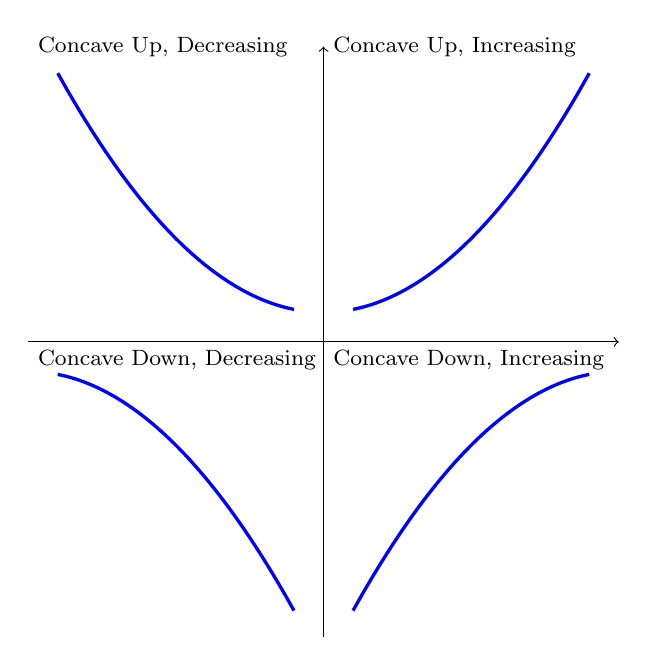
\begin{tikzpicture}[
            scale=1.5,
            declare function={
                func(\x) = \x*\x*0.4;
                Width=5;
                Height=5;
            }
        ]

            \draw[domain=0.25:2.25, smooth, variable=\x, blue, very thick] plot ({\x}, {func(\x - 2.5) + 2.75});
            \draw[domain=2.75:4.75, smooth, variable=\x, blue, very thick] plot ({\x}, {func(\x - 2.5) + 2.75});
            \draw[domain=0.25:2.25, smooth, variable=\x, blue, very thick] plot ({\x}, {-func(\x) + 2.25});
            \draw[domain=2.75:4.75, smooth, variable=\x, blue, very thick] plot ({\x}, {-func(\x - 5) + 2.25});
            
            \node[right] at (0, Height) {\footnotesize Concave Up, Decreasing};
            \node[right] at ({Width / 2}, Height) {\footnotesize Concave Up, Increasing};
            \node[right] at (0, Height / 2 - 0.15) {\footnotesize Concave Down, Decreasing};
            \node[right] at ({Width / 2}, {Height / 2 - 0.15}) {\footnotesize Concave Down, Increasing};
            
            \draw[->] ({Width / 2}, 0) -- ({Width / 2}, Height);
            \draw[->] (0, {Height / 2}) -- (Width, {Height  / 2});
        \end{tikzpicture}
    \end{minipage}
    \begin{minipage}{0.5\textwidth}
        Functions may present \textbf{concavity}
        \hphantom{ } \\
        \begin{itemize}
            \item \(f(x)\) is \textbf{concave up} on an interval \(I\) if all of the tangents on \(I\) are below the graph.
            \item \(f(x)\) is \textbf{concave down} on an interval \(I\) if all of the tangents on \(I\) are above the graph.
        \end{itemize}
        \hphantom{ } \\
        \begin{itemize}
            \item \(f''(x)>0\) for all \(x\) in some interval \(I\) then \(f(x)\) is concave up on \(I\)
            \item \(f''(x)<0\) for all \(x\) in some interval \(I\) then \(f(x)\) is concave down on \(I\)
        \end{itemize}

        This works because when the function is concave up, it increases or decreases more and more. So \(f'(x)\)
        tells us that \(f(x)\) is increasing or decreasing, and \(f''(x)\) tells us the rate at which the increment
        is increasing or the decrease is decrementing. The same goes for when the function is concave down.
    \end{minipage}
\end{snippet}

\begin{snippetdefinition}{inflection-point-definition}{Inflection Point}
    An \textit{inflection point} is a point where the function \(f(x)\) is continuous and the concavity at that point changes.
\end{snippetdefinition}

\begin{snippetproposition}{inflection-point-double-derivative}{}
    If a \function \(f(x)\) has an inflection point at \(x_0\),
    then \(f''(x_0)=0\).
\end{snippetproposition}

\subsection{Second Derivative Test}

\begin{snippet}{second-derivative-test}
Suppose that \(x=c\) is a critical point of \(f(x)\) such that \(f'(x)=0\)
and that \(f''(x)\) is continuous around \(x=c\).
\begin{itemize}
    \item If \(f''(x)<0\) then \(x=c\) is a maximum.
    \item If \(f''(x)>0\) then \(x=c\) is a minumum.
    \item If \(f''(x)=0\) then \(x=c\) could be a maximum, minimum or neither.
\end{itemize}
\end{snippet}

\section{Absolute Extrema}

\begin{snippet}{zero-derivative-not-necessarily-extrema}
    When looking for an absolute extrema in a \function, asking when
    its derivative is zero is not enough since the function may not be continuous
    and have a maxima at a discontinuity point.
\end{snippet}

\end{document}